\documentclass[6pt, spanish]{report}
\usepackage[spanish]{babel}
\selectlanguage{spanish}
\usepackage[utf8]{inputenc}
\usepackage[cp1252]{inputenc}
%\usepackage{amsmath}
\usepackage{amssymb}
\usepackage{graphicx} % Required for including images
\graphicspath{{figures/}} % Location of the graphics files
\usepackage{booktabs} % Top and bottom rules for table
\usepackage[font=small,labelfont=bf]{caption} % Required for specifying captions to tables and figures
\usepackage{amsfonts, amsmath, amsthm, amssymb} % For math fonts, symbols and environments
\usepackage{wrapfig} % Allows wrapping text around tables and figures

\usepackage[svgnames]{xcolor} % Specify colors by their 'svgnames', for a full list of all colors available see here: http://www.latextemplates.com/svgnames-colors

\documentclass[a4paper, 11pt]{article}
\usepackage{comment} % enables the use of multi-line comments (\ifx \fi) 
\usepackage{lipsum} %This package just generates Lorem Ipsum filler text. 
\usepackage{fullpage} % changes the margin

\begin{document}
%Header-Make sure you update this information!!!!
\noindent
\large\textbf{CALENTAMIENTO GLOBAL DE 1.5 ºC} 
\hfill \textbf{Grupo 3} \\
\normalsize
Saavedra Calderón José Ángel
 \hfill Lab Date: 01/27/2018 \\
\hfill Prof. Carlos Lizárraga Celaya

\section*{Introducción}
En la reunión de las partes COP 21, los Acuerdos de París 2015, 195 países acordaron reducir para el final del siglo 21, un 30\% sus emisiones de CO2, el gas tipo invernadero mas abundante y que atrapa el calor radiado por la superficie de la Tierra. Con ello se buscaba no rebasar en 2°C la temperatura promedio global en referencia a la temperatura global en los inicios de la era preindustrial (1840).
A pesar de esto, en el reporte del IPCC en el año 2018 nos arrojo un resultado del impacto de un calentamiento global de 1.5° por arriba de niveles pre-industriales. Con esto se ha experimentado un calentamiento global mayor al promedio en muchas regiones durante diferentes estaciones, calentándose más sobre los continentes que en el océano. 



\section*{Resultados del IPCC}

\subsection*{¿Dónde se encuentra el calentamiento global?}
Con el reporte del IPCC, se obtuvo que el calentamiento global se encuentra en mayor parte distribuido dentro del océano, contando con un 93.4\% de este, como se muestra en la siguiente gráfica:


\begin{center}\vspace{.2cm}
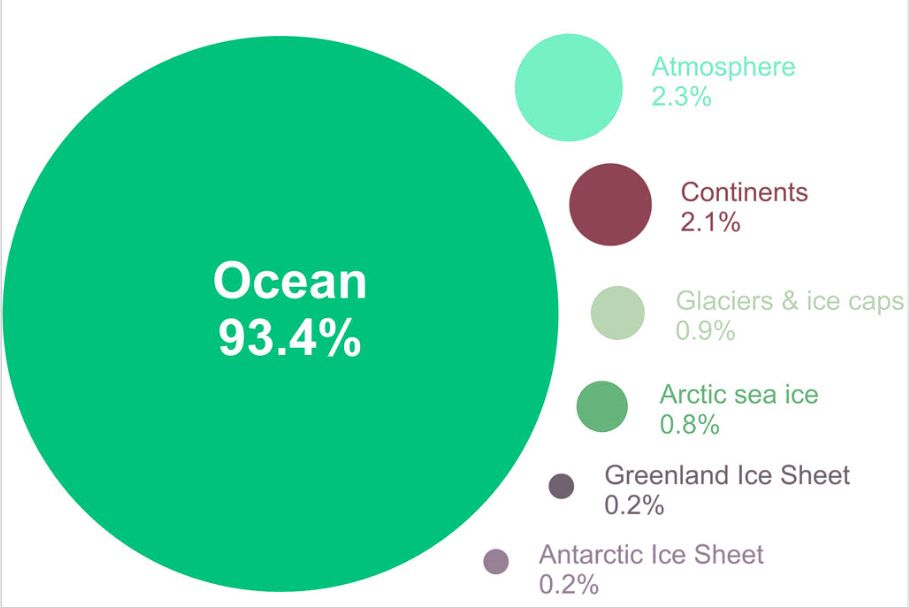
\includegraphics[width=.2\linewidth]{Grafica1.jpg}
\captionof{figure}{\color{Indigo} Concentración del cambio climático. }
\end{center}\vspace{.2cm}



\subsection*{Cambio de temperatura y emisiones de CO_{2}_}
Lo mas impactante del reporte es el resultado y predicciones de lo que sucederá si no tomamos en cuenta nuestras emisiones de CO$_{2}$ y el daño que provocamos con la misma. 
Este mismo reporte nos mostró la siguiente gráfica, en la cual podemos observar el aumento de temperatura que se prevé para los años por venir

\begin{center}\vspace{.2cm}
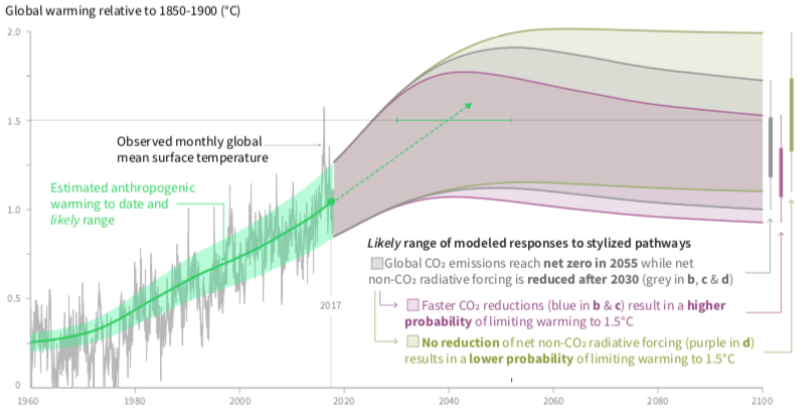
\includegraphics[width=.2\linewidth]{Graficas2.png}
\captionof{figure}{\color{Indigo} Planeación de cambio de temperatura}
\end{center}\vspace{.2cm}


Además del cambio de temperatura, también nos brindaron la producción de CO$_{2}$  

\begin{center}\vspace{.2cm}
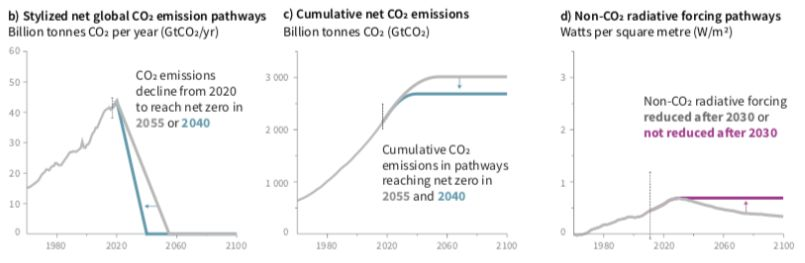
\includegraphics[width=.2\linewidth]{Grafica3.jpg}
\captionof{figure}{\color{Indigo} Generación de $CO_2$ y plantación a un futuro}
\end{center}\vspace{.2cm}


\subsection*{RFCs}
Otro tema importante tratado en el reporte son las RFCs, por sus siglas en ingles RFC (Five Reasons for Concern), siendo los eventos posibles y el impacto que pueden tener en la economía, las personas, y ecosistemas al rededor de diversos sectores y regiones.

\begin{center}\vspace{.2cm}
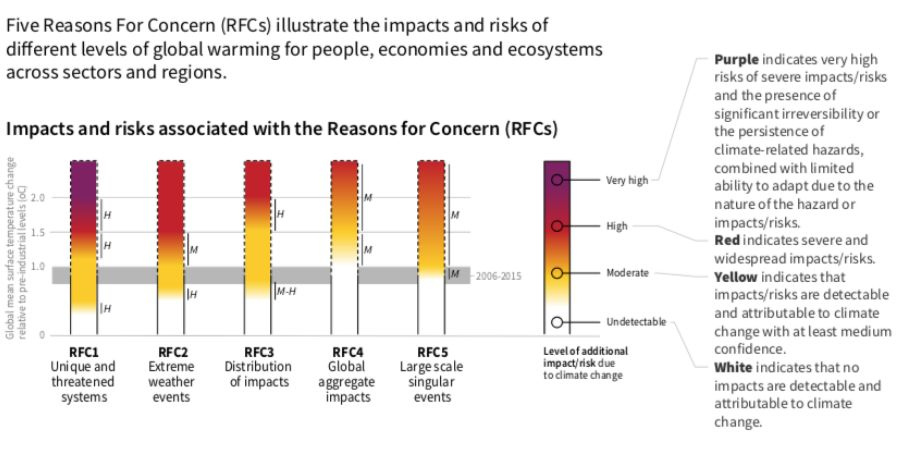
\includegraphics[width=.2\linewidth]{Grafica4.jpg}
\captionof{figure}{\color{Indigo} RFCs. }
\end{center}\vspace{.2cm}
 
Como se puede observar en la imagen, los eventos están ordenados según su impacto, y que tan posible sera no revertir ese resultado, teniendo entonces lo siguiente.

1.Sistema único y amenazado
     
2. Eventos climáticos extremos

3. Distribución de impactos

4. Impactos globales agregados

5. Eventos singulares de larga escala



\section*{Mundo actual}
EL reporte de IPCC también nos brinda una comparación regional y por tiempos de como el calentamiento global se presenta en el mundo. 

\begin{center}\vspace{.2cm}
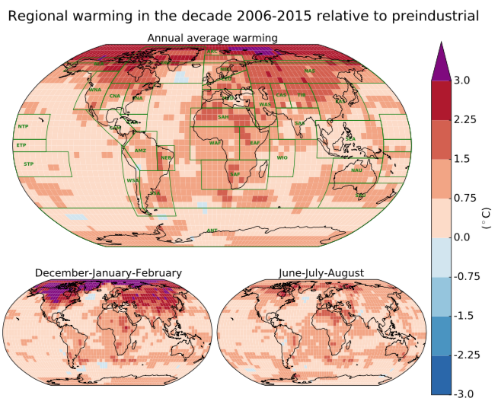
\includegraphics[width=.2\linewidth]{Grafica5.png}
\captionof{figure}{\color{Indigo} Calentamiento global en la década 2006-2015}
\end{center}\vspace{.2cm}

Como podemos observar en la figura 5, el cambio de temperaturas a durante el año se ve mas presente en aquellas ciudades ubicadas por encima del ecuador, siendo esto una clara demostración de como aquellas naciones que se encuentran mas industrializadas son las que mas afectadas se ven. 
Además de eso también se observa que el cambio se nota mas durante invierno.


\begin{center}\vspace{.2cm}
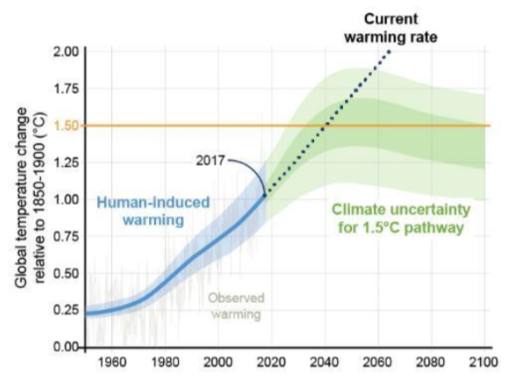
\includegraphics[width=.2\linewidth]{Grafica6.png}
\captionof{figure}{\color{Indigo} Cambio climático en el último siglo}
\end{center}\vspace{.2cm}

En la figura 6 observamos el aumento de temperatura global a través de los años y una proyección a futuras décadas.
Como se observa también se encuentra con una linea que nos marca el punto máximo el cual, al pasarlo, podríamos llegar a ocasionar las situaciones que se repasaron anteriormente en la sección de RFCs. 



\section*{Expectativas}

Terminando el reporte también nos brinda un análisis a futuro de las situaciones a las que se llegarían si continuamos así, al igual que aquello que se llegaría de hacer un cambio drástico a nuestras actividades para favorecer este cambio climático y no pasar de los 1.5°C



\begin{center}\vspace{.2cm}
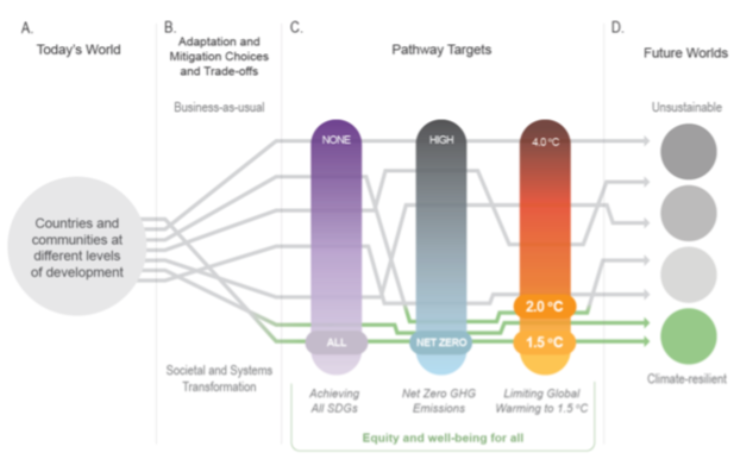
\includegraphics[width=.2\linewidth]{Grafica7.png}
\captionof{figure}{\color{Indigo} Posibles desenlaces 1}
\end{center}\vspace{.2cm}






\begin{center}\vspace{.2cm}
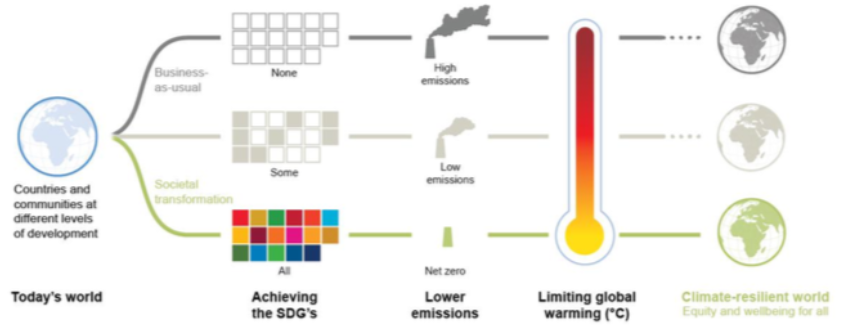
\includegraphics[width=.2\linewidth]{Grafica8.png}
\captionof{figure}{\color{Indigo} Posibles desenlaces 2}
\end{center}\vspace{.2cm}

Tomando como referencia las figuras 7 y 8, vemos los posibles resultados a los que llegamos según el camino que sigamos y que tampoco sustentable sera futuro que podemos aspirar según el camino que tomemos.

 
\section*{Reflexión}
Por ultimo, es importante recalcar la conclusión a la que cualquier persona puede llegar, además de que las naciones involucradas también han llegado a la misma, si seguimos con la misma producción de $C0_2$ como lo hemos estado haciendo hasta el momento en los años por venir estaremos pagando las consecuencias que se tienen planeadas. 
Se ha mencionado ya varias veces, la humanidad se encuentra en un punto critico el cual nos pueda dirigir a una situación de no retorno. 



\begin{thebibliography}{9}
\bibitem{Global warming} Kelly Levin \emph{8 Things You Need to Know About the IPCC 1.5˚C Report}. World Resources Institute. Available from World Wide Web: (https://www.wri.org/blog/2018/10/8-things-you-need-know-about-ipcc-15-c-report).

\bibitem{Global warming} Stephen Leahy \emph{Climate change impacts worse than expected, global report warns}. National Geographic Available from World Wide Web: (https://www.nationalgeographic.com/environment/2018/10/ipcc-report-climate-change-impacts-forests-emissions/).


\bibitem{Global warming} \emph{Global warming report, an 'ear-splitting wake-up call' warns UN chief}. World Resources Institute. Available from World Wide Web: (https://news.un.org/en/story/2018/10/1022492).


\end{thebibliography}

\end{document}
